\chapter{Modelling Semantic Features in Fine-Tuned Vector Spaces}\label{ch5}


\section{Introduction}

%Why are \hmark{document} representations of rankings important in research, society, ML professionals. why is our work needed, how can you use our work
%\hmark{document} representations are typically either sparse but not complex, e.g.\ bag-of-words, or enriched with semantic spatial information that is distributed across dimensions, e.g.\ vector spaces. In this work, we build a \hmark{document} representation that uses the spatial relationships of a vector space to construct a new representation, wherein the dimensions of the representation correspond to rankings on properties, labelled as clusters of words e.g.\ "Horror, Scary, Terrifying" in a domain of movie reviews. We improve the quality of this representation by introducing a post-processing step. Importantly, the entire process is unsupervised, and we show that both our method to obtain a new representation and our post-processing step can be applied to two different kinds of vector spaces, across four different text domains.

%As natural language data increases, as does the need for tools to accurately represent and interpret that data. However, typically representations are either too sparse to be effective for classification, e.g.\ bag-of-words, where each dimension correspends to a word rather than a concept, which in the case of a decision tree may result in many branches and potentially overfit, or vector spaces are used, which contain dimensions that have ambiguous meaning. Despite advances in methods to represent word vectors such that each dimension represents a particular concept, (cite?) there are not many \hmark{document} representations that have both the characteristics of accuracy and independence.% In this work, rather than make a claim of human interpretability, which is ambiguous and difficult to measure, we instead claim that the representation we build contains clearly distinct 

% Give short table of examples to make clear some points?

%There are a number of problems with similarity-based representations. 

%Vector space representations, or `embeddings', play a crucial role in various areas of natural language processing. For instance, word embeddings \cite{DBLP:conf/nips/MikolovSCCD13,glove2014} are routinely used as representations of word meaning, while knowledge graph embeddings \cite{Bordes_translatingembeddings} are used to find plausible missing information in structured knowledge bases, or to exploit such knowledge bases in neural network architectures. In this paper we focus on domain-specific semantic spaces, i.e.\ vector space representations of the objects of a single domain, as opposed to the more heterogeneous setting of e.g.\ word embeddings. 

%Such domain-specific semantic spaces are used, for instance, to represent items in recommender systems \cite{Vasile:2016:MPE:2959100.2959160,liang2016factorization,van2016learning}, to represent entities in semantic search engines \cite{DBLP:conf/sigir/JameelBS17,van2017structural}, or to represent examples in classification tasks \cite{DBLP:conf/iccv/DemirelCI17}. In many semantic spaces it is possible to find directions that correspond to salient features from the considered domain. For instance,  \newcite{gupta2015distributional} found that features of countries, such as their GDP, fertility rate or even level of CO$_2$ emissions, can be predicted from word embeddings using a linear regression model. Similarly, in \cite{kim2013deriving} directions in word embeddings were found that correspond to adjectival scales (e.g.\ bad $<$ okay $<$ good $<$ excellent) while \newcite{DBLP:conf/acl/RotheS16} found directions indicating lexical features such as the frequency of occurrence and polarity of words. Finally, \newcite{derracAIJ} found directions corresponding to properties such as `Scary', `Romantic' or `Hilarious' in a semantic space of movies. 

 %Such feature directions are useful in a wide variety of applications. The most immediate example is perhaps that they allow for a natural way to implement critique-based recommendation systems, where users can specify how their desired result should relate to a given set of suggestions \cite{viappiani2006preference}. For instance, \newcite{Vig:2012:TGE:2362394.2362395} propose a movie recommendation system in which the user can specify that they want to see suggestions for movies that are ``similar to this one, but scarier''. If the property of being scary is adequately modelled as a direction in a semantic space of movies, such critiques can be addressed in a straightforward way. Similarly, in \cite{kovashka2012whittlesearch} a system was developed that can find ``shoes like these but shinier'', based on a semantic space representation that was derived from visual features. Semantic search systems can use such directions to interpret queries involving gradual and possibly ill-defined features, such as ``\emph{popular} holiday destinations in Europe'' \cite{DBLP:conf/sigir/JameelBS17}. While features such as popularity are typically not encoded in traditional knowledge bases, they can often be represented as semantic space directions.  As another application, feature directions can also be used in interpretable classifiers. For example, \newcite{derracAIJ} learned rule based classifiers from rankings induced by the feature directions. Along similar lines, in this paper we will use shallow decision trees to evaluate the quality of our feature directions.

% the directions emerging from a vector space representation are not explicitly learned to model the corresponding properties. 
%For example, we may find a direction corresponding to the property `violent' in a space of movies, which would allow us to approximately rank the movies from the least to the most violent. 
%One limitation of this basic strategy is that when learning vector space representations, there can be a trade-off between preserving similarity structure and having directions which faithfully model salient properties. Since standard methods for learning vector space representations are essentially based on preserving the similarity structure, we argue that a post-processing step is needed to obtain high-quality directions. To this end, we propose a simple neural network model which is aimed at fine-tuning the initial vector space representation w.r.t.\ the chosen interpretable directions. Importantly, the whole process of identifying directions and fine-tuning the vector space remains completely unsupervised, with the neural network being trained based on statistics collected from the bag-of-words representations of the \hmark{document}s. 

% General overview of the problem and motivations

Chapter \ref{ch3} introduced a method to obtain  feature-directions from vector-spaces, as well as methods to test the quality of these feature-directions and their  associated \hmark{\hmark{document}} rankings. Then, this method was applied in Chapter \ref{ch5} to obtain feature-directions from the layers of neural networks. However, feature-directions obtained from either of these vector spaces can sometimes be sub-optimal. For example in the case of neural network auto-encoders, it was found that the quality of feature-directions in \hmark{an} auto-encoder representations degrade the more that the auto-encoder layers are stacked.  

%In Chapter \ref{chapter3} and Chapter \ref{chapter5} it was shown that feature-directions can be obtained from a variety of vector-spaces regardless of how they have been learned, e.g.\ Multi-Dimensional Scaling representations are learned with a similarity-centered objective, and denoising auto-encoder's are learned with an objective to retain information, but feature-directions can be obtained from both of them. However, the feature-directions learned are sub-optimal, as they a consequence of a learning objective rather than being learned with optimal feature-directions being considered. 




% More specific outline of the problem for similarity-centered objectives

 In \hmark{F}igure \ref{fig:toyExample}, a problem that can occur with feature-directions from representations learned with a similarity-\hmark{centered} objective, e.g.\ Multi-Dimensional Scaling (see Section \ref{ch2:MDS}), is illustrated. This is an example problem in the toy domain of shapes, where  basic geometric shapes are embedded in a two-dimensional space. In this example, directions have been identified which encode how light an object is and how closely its shape resembles a square. While most of the shapes embedded in this space are grey-scale circles and squares, one of the shapes embedded in this space is a red triangle, a clear outlier. When considering that the objective the space is learned with \hmark{is based on similarity}, the spatial representation for this triangle  is correct,  as it is far from all the other shapes. However, when ranking the shapes on the feature-directions for square and light, the  outlier  takes up an extreme position on the rankings. This means that the triangle is ranked incorrectly, as it is considered to be the shape that most exhibits the features "light" and "square".

\begin{figure}
	\centering
	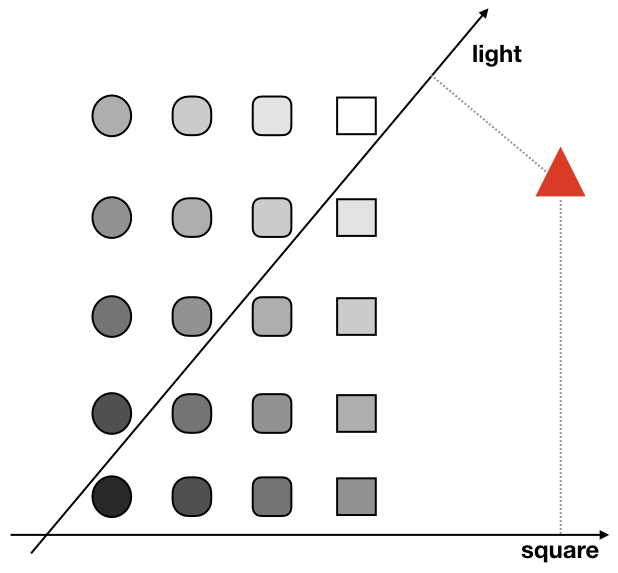
\includegraphics[width=180pt]{images/shapes}
	\caption{Toy example showing the effect of outliers in a two-dimensional embedding of geometric shapes.}
	\label{fig:toyExample}
\end{figure}

Ideally, representations would be learned with knowledge of feature-directions. For example, the method to learn a representation of the toy domain would \hmark{take into account} that it should model the features "square" and "light" rather than a similarity objective, so that this triangle would end up closer to the bottom-left corner. However, as we cannot a-priori determine the features the space must be learned from, it is difficult to learn a representation in this way. This chapter instead introduces an unsupervised method, that given a representation and its associated feature-directions,  can obtain a  vector space and associated feature-directions where the quality of the feature-directions is prioritized  over the similarity structure. The intention of this method is to resolve issues like those described in the previous two paragraphs.

To introduce the idea behind the method, we start with the assumption that each feature-direction is characterised by one feature-word, which describes the feature. \hmark{In other words}, if the feature-ranking of a \hmark{document} on a feature-direction is faithful to the bag-of-words score for the feature-word in the \hmark{document}, then the feature-ranking is good. To give an example of why this assumption is useful, in the Movies domain \ref{datasets:movies} Multi-Dimensional Scaling (MDS) \hmark{space} there is the case of an Indian Bollywood movie that is very unlike other movies, as its reviews only use language specific to Bollywood films and the number of reviews it has is low overall. This movie occupies a top-ranking position in a variety of feature-directions,  as a consequence of it being very dissimilar to other movies. \hmark{This chapter introduces a method that can  solve this problem} by attempting to match its  ranking in the vector space \hmark{that is very high in the initial space}, to its bag-of-words value, which is zero. This results in this  outlier movie being moved down drastically in the rankings. 

To give some  additional examples, in Table \ref{tabTopRanked}, names of \hmark{Place-Types (that correspond to text documents in the Place-Types dataset)} are shown ranked on feature directions \hmark{from their domain} (See Section \ref{datasets:Place-Types}). In these examples, for the cluster-feature $\{\textit{steep},\textit{climb},\textit{slope}\}$, the top ranked \hmark{Place-Type} \textit{mountain} is clearly relevant. However, the next two \hmark{Place-Type}s --- \textit{landscape} and \textit{national park} --- are not directly related to this feature. Intuitively, they are ranked highly because of their similarity to \textit{mountain} in the vector space. Similarly, for the second feature, \textit{building} is ranked highly because of its similarity to \textit{skyscraper}, despite intuitively not having this feature. Finally, \textit{fence} received a high rank for several features,  mostly because it is an outlier in the space. 


\begin{table*}[t]
	
	\centering
	\setlength{\tabcolsep}{14pt}
	\renewcommand{\arraystretch}{1}
	\scriptsize
	\begin{tabularx}{\textwidth}{l l l}
		\textbf{Feature direction} & Highest ranking objects & Highest fine-tuned ranking objects\\
		\toprule             
		\{steep, climb, slope\}                   & mountain, landscape, national park & ski slope, steep slope, slope                                     \\
		\{illuminated, illumination, skyscraper\} & building, city, skyscraper         & tall building, office building, large building                    \\
		\{play, kid, kids\}                       & school, field, fence               & college classroom, classroom, school                              \\
		\{spooky, creepy, scary\}          & hallway, fence, building             & hospital room, hospital ward, patient room                  \\
		\{amazing, dream, awesome\}                   & fence, building, beach    & hotel pool, resort, beach resort \\
		\{pavement, streetlight, streets\}        & sidewalk, fence, building          & overpass road, overpass, road junction                            \\
		\{dead, hole, death\}                     & fence, steps, park                 & grave, cemetery, graveyard                                        \\
		\{spire, belltower, towers\}              & building, arch, house              & bell tower, arch, religious site                                  \\
		\{stones, moss, worldheritage\}           & landscape, fence, steps            & ancient site, ancient wall, tomb                                  \\
		\{mosaic, tile, bronze\}                  & building, city, steps              & cathedral, church, religious site     \\
	
	\end{tabularx}
	
	\caption{Comparing the highest ranking Place-Type objects in the original and fine-tuned space}\label{tabTopRanked}
\end{table*}


Generally, the method that fine-tunes vector spaces and their associated feature-directions is as follows: First, a vector space is learned from bag-of-words representations of the considered \hmark{document}s, using a standard similarity-centric method or neural network. Next, the method from \hmark{C}hapter \ref{ch3} is used to  obtain feature-directions and their associated words from a vector space. Then, following our assumption outlined in the previous paragraph,  \hmark{document}s are ranked on the feature-direction's associated words using the bag-of-words. Finally, this ranking is used to fine-tune the vector space and feature-directions so that the resulting feature-rankings are more faithful to the ranking on the bag-of-words.

% Why does it work? What does it mean?

%This Chapter introduces a post-processing method on vector-spaces to obtain better feature-directions. First, the method described in Chapter \ref{Chapter3} is used to obtain  cluster-directions in a vector space. Then, we obtain a target-ranking  then the  feature-rankings of these directions are improved by shifting them closer to a ranking induced from PPMI scores. 


%In Chapter \ref{Chapter5}  feature directions in a variety of neural network architectures, and how these directions can be used to explain how these networks function was shown. In the case of stacked auto-encoders, however, we noticed that each layer became less and less interpretable.  Even in the case of feedforward networks, which generally remained more interpretable than stacked autoencoders, we noticed a clear drop in Kappa scores. The question we study in this chapter is whether it is possible to take a vector space which is less interpretable than we would like, and manipulate it so it models feature directions in a better way. The intuitive idea is to look at the features which are best represented in the initial vector space, and to fine-tune the representations so they capture these features in a more faithful way. Another way of looking at this is that our proposed method prioritises the interpretable features that are captured by a given vector space, possibly at the expense of other, less interpretable features.

%One way to apply this method is to a representation produced by an auto-encoder, ensuring that it retains key features in the representation while also reducing its size. % Talk about how it doesn't work?
 %Another way of applying this method is to the vector spaces and feature-directions found in Chapter \ref{Chapter3}. These vector space representations were learned with a similarity-centred objective, i.e.\ the main consideration when learning these representations is that similar \hmark{document}s should be represented as similar vectors. An important observation is that such spaces may not actually be optimal for modelling feature directions. 




%For example, \cite{Murphy} found that PCA dimensions did not typically make sense, and FRAGE \cite{Gong2018} achieved state-of-the-art results by removing the bias that a representation has for frequent words. If these biases exist, and the structure is influenced by the similarity such that it does not prioritize a directional structure, then it is unlikely to achieve good results with the method from Chapter 3.

%The aim of this Chapter is to focus the spatial representation on having good directions. This can be understood to be sacrificing similarity information in exchange for direction information. Using the method from the previous chapter,  semantically important feature-directions in a considered domain are determined. Then, from these directions the semantic space and the associated feature directions are fine-tuned to  better rank \hmark{document}s. 



  



This chapter is a follow-up of the previous two chapters, where previously feature-directions are identified in a variety of vector-spaces, and their potential applications are discussed, this chapter focuses on improving the quality of these feature-directions to achieve better results. This chapter continues with explaining the method to fine-tune a vector space and its associated feature directions using a bag-of-words in detail. Afterwards, we show  quantitative results to see how the fine-tuning affects simple interpretable classifiers (as in chapter \ref{ch3}). Finally, we end with a conclusion for potential future work.


%We evaluate our method using one and three depth decision trees. For trees with a single node, we argue that improving the classification score of natural domain tasks, e.g.\ classifying the genre of movies by their reviews, is good evidence that the dimension used to classify the objective contains relevant domain knowledge and is self contained. We find that our fine-tuned representation improves the F1 score of depth-one and depth-three trees, sometimes substantially, and beats our baseline. Additionallly, we find that  often the single depth trees perform well for each class, sometimes even exceeding the depth-three trees. In diagram 1, we give an example of a three depth decision tree from a domain of movie reviews, used to classify the \hmarkn{`}Horror' genre. % Just an example



%We find that our fine-tuned representation consistently improves depth-one and depth-three decision trees, sometimes substantially. Additionally, we find that the single depth trees perform well for many classes, often performing on par with, or even better than larger decision trees. 

%The remainder of the paper is structured as follows. After presenting related work in the next section, Section \ref{LearningInterpretableDirections} explains how interpretable directions are identified from the initial vector space, while Section \ref{secFinetuning} introduces our proposed fine-tuning method. Finally, in Section \ref{secExperiments} we present our experimental results, showing that decision trees learned from the fine-tuned rankings perform we
%In our work, we aim to obtain a fine-grained, conceptually sound interpretable representation in an entirely unsupervised way. We follow previous work, where authors \cite{Derrac2015} used an unsupervised method to obtain fine-grained interpretable rankings of entities from a vector space wherein entities correspond to points, and concepts to regions e.g.\ in a vector space learned from wine tasting notes, a ranking of wines based on how many $'tannins'$ they have. They did this by finding highly separable terms e.g.\ in a space learned from movie reviews, $'scary'$, $'funny'$,  $'romantic'$, and a corresponding direction for each of these terms. These directions were then clustered together  $'scary'$, $'gory'$, $'terrifying'$ using a simple K-means algorithm. Finally, a ranking was induced for each entity on each cluster (e.g.\ a ranking of how $'scary'$ each movie is), and used as input to an interpretable classifier, e.g.\ a Decision Tree classifying the genre of a movie. See Fig 1.

%\begin{figure*}
%\includegraphics[scale=0.3]{horror-ndcg-finetune.png}
%\centering
%\caption{A Decision Tree obtained using our process that classifies if a movie is in the "Horror" genre.}
%\end{figure*}

%Previously, authors  \cite{Steven} used an unsupervised method to represent semantic relationships learned in a vector space in the form of fine-grained interpretable rankings of \textit{entities}, e.g.\ in a vector space learned from \textit{wine} tasting notes, a ranking of \textit{wines} based on how many $'tannins'$ they have. In their work, they learned a vector space wherein entities are points in the space, and concepts are regions. Then, they obtained a hyperplane that separates entities for each term, scored by separability. Highly separable terms we can understand correspond to natural concepts (e.g.\ in a space learned from movie reviews, $'scary'$, $'funny'$,  $'romantic'$). From these hyperplanes, we can obtain their orthogonal directions, and then induce a ranking of entities on this direction by obtaining the dot product of the entity points on the direction vectors (e.g.\ a ranking of how $'scary'$ each movie is). These directions can be clustered together by similarity e.g.\ $'scary'$, $'gory'$, $'terrifying'$, and used as input to an interpretable classifier.

%In our work, we learn fine-grained interpretable features that better represent natural concepts in the domain, by describing the representation of the relationship between entities more accurately in the domain, and validate that our model performs greater than previous methods by learning shallow decision trees, see figure 1.

%What are other approaches? What is our approach? Why is it important?

%What previous  work are we building on? Why is this information important? How does it fit into our work? How does it separate from our work?

%Previously, authors  \cite{Steven} used an unsupervised method to represent semantic relationships learned in a vector space in the form of fine-grained interpretable rankings of \textit{entities}, e.g.\ in a vector space learned from \textit{wine} tasting notes, a ranking of \textit{wines} based on how many $'tannins'$ they have. In their work, they learned a vector space wherein entities are points in the space, and concepts are regions. Then, they obtained a hyperplane that separates entities for each term, scored by separability. Highly separable terms we can understand correspond to natural concepts (e.g.\ in a space learned from movie reviews, $'scary'$, $'funny'$,  $'romantic'$). From these hyperplanes, we can obtain their orthogonal directions, and then induce a ranking of entities on this direction by obtaining the dot product of the entity points on the direction vectors (e.g.\ a ranking of how $'scary'$ each movie is). These directions can be clustered together by similarity e.g.\ $'scary'$, $'gory'$, $'terrifying'$, and used as input to an interpretable classifier.

%Granular rankings lead to more fine-grained control, meaning that sensitive issues can be resolved granularly.

%What is our work? What is the novelty of the contribution? How does it affect the results? In what ways is it better? 

% So our work is about learning a more accurate representation following Steven's work

%We introduce an unsupervised method to improve the accuracy of salient directions, by using them as scikit-learns in a neural network, that trains these directions to be closer to their bag-of-words representation, while maintaining fidelity to the original rankings. To test these rankings, we then use them as the input to a low-depth decision tree, which we use as a quantitative measure to show that our features are more accurate and interpretable than both a Latent Dirchlet Allocation (LDA) baseline and previous work. We evaluate our work in three different domains, movie reviews, flickr tags describing Place-Types, and the 20 Newsgroups dataset.

%The rest of this paper is organized as follows. Section 2 describes related literature, Section 3 describes previous work in more detail that we use to obtain directions and rankings, Section 4 describes our work, Section 5 details our experiments and we conclude the work in Section 6. 

%
%\section{Related Work}

% Other approaches offer different ways of attacking the same problem
% Topic models give statistical models, additionally leveraging labelled data or relaxing/adding constraints

%-------------
% Interpretability, other approaches to interpretability
% Our approach to interpretability, specifically text representations ala: PCA, Sparse PCA,
% LDA, 
% NMF,
% Word vectors, sparsity applications
% Final statement clarifying differences and setting up the description of our work
%-------------

%One method in particular has achieved global explanations \cite{Lakkaraju2017}, by obtaining decision sets that approximate an existing model. 

% Something about linear models?

% Topic models




%The most commonly used representations for text classification are bag-of-words representations, topic models, and vector space models. Bag-of-words representations are often too simplistic and sparse to perform well, unless a bag of word vectors is used, or tailored to the domain in some way. Topic models and vector space models are two alternative approaches for generating low-dimensional \hmark{document} representations.

%\textbf{Topic models.} 
%Similarly, our feature directions are also labelled with the most closely associated words. 
%However, while LDA only uses bag-of-words (BoW) representations, our focus is specifically on identifying and improving features that are modelled as directions in semantic spaces. 


%where \hmark{document}s are represented by a distribution of topics, and each topic is a distribution over words \cite{Blei2003}.  By simply taking the words with the top probability for a topic, we can easily obtain coherent topics. 
%removed a bunch of stuff about \hmark{document} classification
%LDA has been extended by many approaches, e.g.\ aiming to avoid the need to manually specify the number of topics \cite{teh2005sharing}, modelling correlations between topics \cite{Blei2006}, or by incorporating meta-data such as authors \cite{rosen2004author} or time stamps \cite{wang2006topics}.

%Topic models and our work, on the surface, produce similar results, as both representations result in distinct dimensions or topics, with \hmark{document}s having an associated numerical value for these topics. However, our method differs in the way these dimensions are obtained, in particular as we rely on the directions in a vector space rather than the raw bag-of-words, our method has the applicability to make use of specialist vector space representations tailored to an objective, e.g.\ a hidden layer output representation obtained from an Long-Short Term Memory network trained to classify sentiment, with very little adjustment.
%Broadly speaking, in the context of \hmark{document} classification, the main advantage of topic models is that their topics tend to be well separated and easy to make sense of, while vector space models tend to be more flexible in the kind of meta-data that can be exploited. The approach we propose in this paper aims to combine the best of both worlds, by providing a way to derive representations with distinct labelled dimensions from vector space models.


%\textbf{Vector space models} typically use a form of matrix factorization to obtain low-dimensional \hmark{document} representations. By far the most common approach is to use Singular Value Decomposition \cite{ASI:ASI1}, although other approaches have been advocated as well. 
%One approach which is of particular interest is non-negative matrix factorization (NMF), in which dimensions correspond to a non-negative combination of words. This is assumed to help interpretability as it means that dimensions can essentially be viewed as topics (i.e.\ they also correspond to scikit-learned sets of words). 

%Instead of matrix factorization, another possible strategy is to use a neural network or least squares optimization approach. This is commonly used for generating word embeddings \cite{DBLP:conf/nips/MikolovSCCD13,glove2014}, but can similarly be used to learn representations of text \hmark{document}s \cite{DBLP:journals/corr/DaiOL15,van2016learning,DBLP:conf/sigir/JameelBS17}. Such approaches have the advantage that various forms of domain-specific structured knowledge can easily be taken into account. Some authors have also proposed hybrid models, which combine topic models and vector space models. For example, the Gaussian LDA model represents topics as multivariate Gaussian distributions over a word embedding \cite{DBLP:conf/acl/DasZD15}. Beyond \hmark{document} representation, topic models have also been used to improve word embedding models, by learning a different vector for each topic-word combination \cite{DBLP:conf/aaai/LiuLCS15}.

%\smallskip
%\noindent \textbf{Fine-tuning embeddings.} Several authors have looked at approaches for adapting word embeddings. One possible strategy is to change how the embedding is learned in the first place. For example, some approaches have been proposed to learn word embeddings that are better suited at capturing sentiment \cite{tang2016sentiment}, or to learn embeddings that are optimized for relation extraction \cite{DBLP:conf/conll/HashimotoSMT15}.
%Other approaches, however, start with a pre-trained embedding, which is then modified in a particular way. For example, in \cite{faruqui2015retrofitting} a method is proposed to bring the vectors of semantically related words, as specified in a given lexicon, closer together. Similarly \cite{yu2017refining} propose a method for refining word vectors to improve how well they model sentiment. In \cite{labutov2013re} a method is discussed to adapt word embeddings based on a given supervised classification task.

%Another way of approaching interpretability is non-negative matrix factorization. NMF has been applied to word vectors \cite{Murphy}, obtaining word-representations (NNSE) that are both accurate and interpretable. Fyshe \cite{Fyshe} also obtained interpretable and accurate representations by adding an additional compositionality constraint to NNSE in order to represent phrasal semantics. 

%Another way of representing text is to learn vectors for each word, by learning distributions from their context. This approach, popularized by GloVe and word2vec have achieved great results in real world applications like entity recognition, semantic role labelling and syntactic parsing \cite{Chen2014,Chen2014b,Guo2014}.    The idea of learning a distribution based on context has also been applied to sentences \cite{Liu2017}, paragraphs and \hmark{document}s \cite{Le2014} with to obtain \hmark{document} representations that perform well at classification tasks. However, these Paragraph Vectors have much less interpretable dimensions \cite{Le2014}.



% Paragraph on word vectors
%Distributional representations of words learned using contextual information have achieved state-of-the-art for many tasks. 




%-------------
% LDA
% LDA for \hmark{document} classification
% Unsupervised LDA approaches
% Supervised (relevant?) LDA approaches
%-------------

% An effective state-of-the-art representation learned using neural networks are word vectors
% Word vectors are effective at representing important concepts, and show high separability
% Further, they've been applied to \hmark{document}s effectively, and show high performance there too.
% However, these standard representations are not very interpretable.
% That's why some authors have applied sparsity and non-negativity constraints to a matrix factorization process
% For \hmark{document}s too
% Mostly, that's how word vectors have been used to obtain an interpretable representation, and like ours, they aim to be both accurate and interpreatble. However, we do not leverage contextual inforamtion in our learning process, instead relying on the raw meaning of each word to improve a set of rankings.

%Recently, a "bag-of-concepts" was also introduced, where word-vectors were clustered and averaged to form a concept. These are particularly relevant to our work, as we also obtain rich representations of words in the form of rankings and cluster them together to form a salient concept. 
%NOTE: This ^ seems like a common approach labelled "bag-of-clusters" for supposed novelty
%Further, there have been representations that combine the power of word vectors and topic models together. \cite{X} and \cite{bibid} did XXXX YYYY, and \cite{bibid} obtained an interpretable \hmark{document} representation that used both.


%-------------
% NMF
% Variations of NMF
% Word vectors, Variations on word vectors for sentences/paragraphs
% Sparse word vectors
% Sparse \hmark{document} vectors
%-------------

%An alternative was introduced by \cite{IDK} as a "bag-of-concepts", where word vectors are clustered together and averaged.   ### This work seemed to be aready done essentially ### Our work is similar in the sense that we cluster together semantic representations of words, but we instead represent words as concepts and a group of words as a direction and associated ranking. Some recent approaches have combined the use of both topic-models and word-vectors, attempting to leverage contextual information to learn better topics or words in a "two-step" process, or combine both procedures together into a single model. Other works that use structural information as part of their learning process to learn an interpretable representation are , who used the structural information of sentences in combination with an attention mechanism to produce \hmark{document} representations with interpretable intermediate structures. 





%have been argued to be less interpretable, and instead a "bag-of-concepts" - has been used, clustering multiple word-embeddings together into concepts, and then using those now interpretable features to classify \hmark{document}s \cite{Kim2017}. We can understand the previous work \cite{Steven}   to be most similar to clustering multiple word-embeddings together, as they also obtain interpretable features from a cluster of properties. However, our work obtains interpretable features from an existing representation, rather than learning a more accurate or interpretable representation. 

%Supervised approaches use labelled data to make a models probabilities more suitable for classification, for example \cite{VanLinh2017} have used supervised data to train a topic model for \hmark{document} classification. %Stuff about unsupervised methods.

%Recently, 'Representation Learning' \cite{Bengio2012} with neural networks have learned text representations that are 'disentangled', meaning that natural domain concepts are well separated in the space.



%Other approaches have looked at combining the structural information of the text into the representation to make it more interpretable.

%However it seems to have potential for producing the kind of 'conceptual space' that the original work derived their inspiration for a vector space to derive semantic relationships from \cite{Bechberger}. 





%Another approach to obtaining a better interpretable classifier is to learn a linear model using an existing black-box model. These approaches are limited to the black-box model they are learning from, and are sometimes reliant on a certain kind of neural network or feature representation. 

%The importance of the salient features of the domain being distinguished from each other has been recognized across many different domains. The most common way of determining these features is understanding what the dimensions of vectors mean, in the context of word vectors this has been achieved by obtaining high-scoring words for the particular dimension and a high-scoring word from another dimension. Being able to judge the difference essentially tests how interpretable the dimension is.

%Our method does not rely on the model and is not totally independent from it. We essentially rely on a good representation that has disentangled the natural features of the domain, and attempt to achieve that by tuning the representation towards a natural classification task. Further, we are not particularly interested in an explanation of the neural network model, rather we want to obtain interpretable features that correspond to natural domain concepts so we can build an interpretable classifier from these features. 


% Might be valuable, but from 2013...
%The quality of a vector space representation has been described as the extent to which semantic concepts are well separated in the space \cite{Bengio2013}, and the ability to obtain these 'disentangled' spaces using neural networks has been widely explored. 


%Typically, rankings of entities are based on features from a knowledge base \cite{Schuhmacher2015}. However, we are interested in improving rankings derived from directions in our space. To do so, we use a novel kind of neural network that outputs the rankings of the clusters and trains them to be closer to the original PPMI values. We can consider this to be fine-tuning the space to become more interpretable. Other works have focused on guiding the hidden layer representation of the network to obtain better rules,  Similar to the concept of improving the space dependent on important features \cite{Chen2016} learns a representation by maximizing the mutual information between a small subset of latent variables that are relevant to a classification task. This method is a form of representation learning, where the representation learned has disentangled the space such that the natural clusters in the data form. However, the variables chosen to be tuned for this method were hand-selected, while the features we tune are obtained in an unsupervised way. Not only that, but we are not necessarily interested in disentangling the space, rather we are interested in a space that can create better rankings so we can use them as the input to an interpretable classifier. 



%Recently, methods to obtain explanations from neural networks by perturbing the inputs and observing the changes to the outputs have risen to prominence as a method to interpret classification decisions. LIME \cite{Ribeiro2016}  obtains a method that can explain the decision of any classifier.  This approach can build trust for the prediction of any classifier, but does not explain the building blocks that lead to the solution. In contrast, our approach makes explicit the semantic relationships that it builds on for classification, and describes meaningful rankings of entities according to these relationships. Some methods, similar to ours, rely on a text-based neural network to function. In \cite{Lei2016}, pieces of input text are extracted to justify predictions, while in \cite{Li2016} the effects of erasure are used to analyse and interpret decisions. However, these methods often do not give the whole picture.  By producing an interpretable classifier, both the prediction is explained and the knowledge of how the classifier has understood the problem is explained. Even though hard to interpret models generally have higher accuracy, it can be difficulty to improve the accuracy of the model based on an explanation of the output alone. In contrast, all information used by the classifier, including its decisions in the trained model, can be both understood and controlled by the user. Further, an interpretable classifier derived from the hidden layer of a network that is classifying the same objective can serve as an explanation of the main concepts learned by the network, with the additional benefit of being able to classify new information in an interpretable way.

%Similar to obtaining interpretable features, obtaining intepretable rules from neural networks has also been previously explored. The existing neural network rule extraction algorithms can be categorized as either decompositional, pedagogical or eclectic \cite{Andrews1995a}. Decompositional approaches derive rules by analysing the units of the network, while pedagogical approaches treat the network as a black box, and examine the global relationships between inputs and outputs. Eclectic approaches use elements of both decompositional and pedagogical approaches. The algorithm in \cite{Kim2000} is a decompositional approach that applies to a neural network with two hidden layers. It uses hyperplanes based on the scikit-learn parameters of the first layer, and then combines them into a decision tree. Our method is similar in that it also uses hyperplanes to obtain property directions, but we provide an unsupervised and more large-scale approach for text-classification, that results in interpretable rankings. NeuroLinear \cite{Setiono1997c} is a decompositional approach applied to a neural network with a single hidden layer that discretizes hidden unit activation values and uses a hyperplane rule to represent the relationship between the discretized values and the first layer's scikit-learns. HYPINV \cite{Saad2007b} is a pedagogical approach that calculates changes to the input of the network to find hyperplane rules that explain how the network functions.



%\section{Identifying Feature Directions}\label{LearningInterpretableDirections}


%We assume that a domain-specific semantic space is given, and that for each of the objects which are modelled in this space, we also have a BoW representation. 
%Our overall aim is to find directions in the semantic space that model salient features of the considered domain. For example, given a semantic space of movies, we would like to find a direction that models the extent to which each movie is scary, among others. Such a direction would then allow us to rank movies from the least scary to the most scary. We will refer to such directions as \emph{feature directions}. Formally, each feature direction will be modelled as a vector $v_f$. However, we refer to \emph{directions} rather than \emph{vectors} to emphasize their intended ordinal meaning: feature directions are aimed at ranking objects rather than e.g.\ measuring degrees of similarity. In particular, if $o$ is the vector representation of a given object then we can think of the dot product $v_f \cdot o$ as the value of object $o$ for feature $f$, and in particular, we take $v_f \cdot o_1 < v_f \cdot o_2$ to mean that $o_2$ has the feature $f$ to a greater extent than $o_1$.

%To identify feature directions, we use a variant of the unsupervised method proposed in \cite{derracAIJ}, which we explain in this section. In Section \ref{secFinetuning}, we will then introduce our approach for fine-tuning the semantic space and associated feature directions. 


%\smallskip
%\noindent \textbf{Step 1: Generating candidate feature directions.} Each feature will be associated with a cluster of words, which we can regard as a description of the intuitive meaning of that feature. Since we assume no \emph{a priori} information about which words might describe features that can be modelled as directions in the vector space, the method initially considers all nouns and adjectives that are sufficiently frequent in the BoW representations of the objects as candidate feature labels. Then, for each considered word $w$, a logistic regression classifier is trained to find a hyperplane $H_w$ in the semantic space that separates objects which contain $w$ in their BoW representation from those that do not. The vector $v_w$ perpendicular to this hyperplane is then taken as the direction that models the word $w$. 
%Let $o_1$ and $o_2$ be the vector representations of two objects. If $v_w$ models the word $w$ well, we would expect that $v_w \cdot o_1 < v_2 \cdot o_2$ if the word $w$ is more strongly related to $o_2$ than to $o_1$. For example, in a space of movies, if $w$ is the word `scary', then we would expect $v_w$ to rank the movies according to how scary they are. 

%\smallskip
%\noindent \textbf{Step 2: Filtering candidate feature directions.} To determine whether the word $w$ is likely to describe an important feature for the considered domain, we then evaluate the quality of the candidate feature direction $v_w$. For example, we can use the classification accuracy to evaluate the quality in terms of the corresponding logistic regression classifier: if this classifier is sufficiently accurate, it must mean that whether word $w$ relates to object $o$ (i.e.\ whether it is used in the description of $o$) is important enough to affect the semantic space representation of $o$. In such a case, it seems reasonable to assume that $w$ describes an important feature for the given domain. 

%One problem with accuracy as a scoring function is that these classification problems are often very imbalanced. In particular, for very rare words, a high accuracy might not necessarily imply that the corresponding direction is accurate. For this reason, \newcite{derracAIJ} proposed to use Cohen's Kappa score instead. In our experiments, however, we found that accuracy sometimes yields better results, so rather than fix the scoring function, we keep this as a hyperparameter of the model that can be tuned. 

%In addition to accuracy and Kappa, we also consider Normalized Discounted Cumulative Gain (NDCG). 
%This is a standard metric in information retrieval which evaluates the quality of a ranking w.r.t.\ some given relevance scores \cite{jarvelin2002cumulated}.  In our case, the rankings of the objects $o$ are those induced by the dot products $v_w \cdot o$ and the relevance scores are determined by the Pointwise Positive Mutual Information (PPMI) score $\textit{ppmi}(w,o)$, of the word $w$ in the BoW representation of object $o$ where
%$\textit{ppmi}(w,o) = \max \big(0, \log\big(\frac{p_{wo}}{p_{w*} \cdotp p_{*o}}\big)\big)$, and
%\begin{align*}
%p_{wo} &= \frac{n(w, o)}{\sum_{w'} \sum_{o'} n(w', o')}
%\end{align*}
%where $n(w,o)$ is the number of occurrences of $w$ in the BoW representation of object $o$, $p_{w*} = \sum_{o'} p_{wo'}$ and $p_{*o} = \sum_{w'} p_{w'o}$.
%In principle, we may expect that accuracy and Kappa are best suited for binary features, as they rely on a hard separation in the space between objects that have the word in their BoW representation and those that do not, while NDCG should be better suited for gradual features. In practice, however, we could not find such a clear pattern in the differences between the words chosen by these metrics despite often finding different words.




%While the Kappa metric was found to perform well, one drawback is that it does not actually evaluate the ranking of the \hmark{document}s induced by $v_w$. To address this, in this paper we will also consider the normalized discounted cumulative gain (NDCG) metric \cite{jarvelin2002cumulated} and, following good results, the accuracy metric. 
% ???? SHOULD WE TALK ABOUT NDCG? NOT SURE IF RESULTS ARE GOOD ????




%\smallskip
%\noindent \textbf{Step 3: clustering candidate feature directions.}
%As the final step, we cluster the best-scoring candidate feature directions $v_w$. Each of these clusters will then define one of the feature directions to be used in applications. The purpose of this clustering step is three-fold: it will ensure that the feature directions are sufficiently different (e.g.\ in a space of movies there is little point in having \emph{funny} and \emph{hilarious} as separate features), it will make the features easier to interpret (as a cluster of terms is more descriptive than an individual term), and it will alleviate sparsity issues when we want to relate features with the BoW representation, which will play an important role for the fine-tuning method described in the next section.

%As input to the clustering algorithm, we consider the $N$ best-scoring candidate feature directions $v_w$, where $N$ is a hyperparameter. To cluster these $N$ vectors, we have followed the approach proposed in \cite{derracAIJ}, which we found to perform slightly better than $K$-means. The main idea underlying their approach is to select the cluster centers such that (i) they are among the top-scoring candidate feature directions, and (ii) are as close to being orthogonal to each other as possible. We refer to \cite{derracAIJ} for more details. 
%To cluster these $N$ vectors, we have used a version of} the standard $K$-means clustering algorithm for this purpose, \blue{where cosine similarity is used instead of Euclidean distance}.  
%The output of this step is a set of clusters $C_1,...,C_K$, where we will identify each cluster $C_j$ with a set of words.
%We will furthermore write $v_{C_j}$ to denote the centroid of the directions corresponding to the words in the cluster $C_j$, which can be computed as $v_{C_j}= \frac{1}{|C_j|} \sum_{w_l\in C_j} v_l$ provided that the vectors $v_w$ are all normalized. These centroids $v_{C_1},...,v_{C_k}$ are the feature directions that are identified by our method. 

%Table \ref{tabKappaNDCG} displays some examples of clusters that have been obtained for three of the datasets that will be used in the experiments, modelling respectively movies, Place-Types and newsgroup postings. For each dataset, we used the scoring function that led to the best performance on development data(see Section \ref{secExperiments}). Only the first four words whose direction is closest to the centroid $v_C$ are shown.

%Selected from using the top-scoring depth-3 tree parameter variations on development data. IMDB Sentiment omitted as it is similar to movie reviews. We find that different scoring-types find different kinds of properties. In this case, we can see that NDCG in particular has found quite specific, almost somewhat niche clusters that correspond to specific types of movies, while the kappa-scored terms are more general and easy to grasp.

%The clusters are assumed to correspond to the most salient properties from the domain of interest. In \cite{derracAIJ} these properties were used to generate commonsense ``a fortiori'' rules of the form ``if $X$ is a Thriller movie and $Y$ is \emph{more scary} than $X$, then $Y$ is a Thriller movie as well'', where `Thriller movie' corresponds to the class that we want to predict and `scary' in this case is one of the properties that was identified from the vector space. In this paper, we will evaluate the usefulness of such properties as features for learning small and interpretable decision trees. 




%When obtaining properties, we only consider terms that have occurred in at least 100 entities for the movies, 50 entities for the Place-Types and 30 entities for the newsgroups. Additionally, we did not include terms that were included in more than $|E| - 10$ entities. These thresholds were chosen such that the amount of terms were roughly equivalent to the datasets chosen in the previous work, resulting in 6335 terms for the newsgroups, 27385 terms for the movies, and 21836 terms for the Place-Types. 

% NOTE: These are copy pasted from past workshop paper. Probably need some changes


%\paragraph{Identifying directions for frequent terms.} To discover terms that correspond to interpretable properties in the MDS space, the nouns and adjectives that occur in sufficiently many reviews are converted to a binary bag-of-words representation and used as input to a linear Support Vector Machine (SVM)\footnote{\url{http://scikit-learn.org/stable/modules/generated/sklearn.svm.LinearSVC.html}}. The SVM is trained to find the hyperplane that best separates the entities that contain the term at least once in their associated textual description. To accommodate class imbalance, we increase the cost of positive instances such that their scikit-learn is inversely proportional to how many times the term has occurred. To assess the quality of the hyperplane found by the SVM, we use Cohen's Kappa score \cite{cohen1960}\footnote{\url{http://scikit-learn.org/stable/modules/generated/sklearn.metrics.cohen_kappa_score.html}} which evaluates how well the hyperplane separates positive/negative instances while taking class imbalance into account. We consider terms with a high Kappa score to be labels of properties that are modelled well by the MDS space. The direction corresponding to a given term/property is given by the vector perpendicular to the associated hyperplane. This vector in turn allows us to determine a ranking of the entities, according to how much they have the  property being modelled. This ranking is obtained by determining the orthogonal projection of each entity on an oriented line with that direction. It is easy to see that if $v$ is the vector modelling a given property, then entity $e_1$ is ranked before entity $e_2$ iff $e_1 \cdot v < e_2 \cdot v$. Another way to look at this is that entities are ranked according to their signed distance to the hyperplane.

%\paragraph{Improving the scoring method.} In the method described by \cite{Derrac2015}, the quality of a property was determined by how well entities that have a property were separated in a space, measured using the Kappa score. We can expect this method to find more "binary" properties, e.g.\ a film will either have gore, or not have any gore at all. In-order to find other kinds of properties, we can instead use a metric that measures how well a direction $d_{t}$ is modelled in the space directly. To do this, we use Normalized Discounted Cumulative Gain (nDCG) \cite{Words2002}\footnote{\url{https://gist.github.com/mblondel/7337391}} to measure the quality of the ranking induced from the direction. This method takes relevance scores for each entity, and a ranking, and outputs an nDCG score for how effective the ranking is at matching those relevance scores, with a greater scikit-learn for those entities that are higher up in the ranking. As the PPMI scores are sparse, this means that many of the entities that are relevant but have a PPMI score of 0 do not make much of an impact on the overall score, essentially allowing us to compare the rankings of those entities that do have an associated PPMI score more effectively than if we had scikit-learned each position equally. The rankings $r$ we evaluate are the ones induced from the direction $d_{t}$, which we obtain from the dot product of the entity vector on the property direction $rank(e, d_{t})$, and we use the PPMI values as the relevance scores $ppmi(e, t)$, under the assumption that they correspond to a good baseline for what we consider to be important for an entity. 
% Taken directly from the journal paper
%\begin{align*}
%\text{DCG}_{r}^{t} &= \sum_{i=1}^{p}\frac{\textit{ppmi}_{i}^{t}}{log_{2}(i + 1)} \\
%\text{IDCG}_{r}^{t} &= \sum^{|\textit{entities}|}_{i=1} \frac{2^{\textit{ppmi}_{i}^{t}}-1}{log_{2}(i + 1)} \\
%\text{nDCG}_{r}^{t} &= \frac{\text{DCG}_{r}^{t}}{\text{IDCG}_{r}^{t}}
%\end{align*}  

%To define nDCG, we can first define Discounted Cumulative Gain (DCG), where $p$ is equal to a position in the ranking of entities on a direction $d_{t}$, and $ppmi_{p_{i}}^{t}$ is equal to the PPMI score for a term at position $i$ in the ranking. Then, we can define the Ideal Discounted Cumulative Gain (IDCG), which is the best possible DCG for a position $p$, where $|entities|$ are the entities for the term ordered by their relevance up to position $p$. nDCG is then simply the DCG normalized by the iDCG.  %Below, we show the top 20 highest scoring properties that are not in the top 100 properties when using the other scoring method. As there are a few duplicates between both methods, this is simply to highlight the different kinds of properties each one obtains.


%By examining these properties, we can see that there are a few distinct kinds of properties. On the Kappa score side, there are specific aspects of technology, e.g.\ blu, meaning blu-ray, vhs, referring to older methods of storage, as well as transfer. These are markedly absent in NDCG, assumedly because they are so binary - a movie is either on vhs or not on vhs. On NDCG's side, we begin to see more informative properties. "prison", "musicals" "western" are all very useful for classifying the type of movie. However, NDCG also finds an interesting somewhat unique collection of propertioes "Branaghs" "astaire" and "crawford" are all names, relating to the movie industry in some way. 

% Deleted stuff by accident here.} These properties are informative, but often repetitive and are sometimes difficult to understand without additional context. In-order to obtain meaningful directions, we can cluster together salient properties to obtain a cluster of terms $c = \{t_{1},  ... , t_{n}\} $, that correspond to a single cluster direction. We first choose the number of clusters equal to the number of dimensions. To determine the cluster centers, we first select directions whose associated Kappa score is above some threshold $T^+$. We  use the highest scoring direction as the center of the first cluster and find the most dissimilar direction to the first cluster's direction to get the centre of the second cluster. Continuing in this way, we repeatedly select the direction which is most dissimilar to all previously selected clusters. By doing so, we obtain a collection of cluster centres that capture a wide variety of different properties from the space. We then associate each remaining direction to its most similar cluster centre. In this step, past work considered  directions whose associated Kappa score is at least $T^-$, where typically $T^-<T^+$. However,  Finally, we take the average of all directions in a cluster to be the overall direction for a cluster. The value of $T^+$ should be chosen as large as possible (given that the terms with the highest Kappa scores are those which are best represented in the space), while still ensuring that we can avoid choosing cluster centers which are too similar. 



%************************************************************************************************
\section{Fine-Tuning Vector Spaces and their Associated Feature Directions}\label{secFinetuning}


%This is essentially re-organizing the space so that feature-directions are prioritized. However, it is important that what was learned in the space is not forgotten. This is why feature-rankings are trained to be more faithful to the PPMI ranking, not to exactly match it. 


%Standard dimensionality reduction methods such as singular value decomposition or Multi-Dimensional Scaling (MDS) aim to learn a vector space that preserves, as much as possible, the similarity structure between the considered text \hmark{document}s. However, for our purposes, the quality of the rankings induced by the interpretable directions is more important than the overall similarity structure. 


To improve the directions and \hmark{address the problems described in the previous section}, we propose a method for fine-tuning the semantic space representations and corresponding feature directions. First, it is explained how to obtain target rankings from PPMI scores. Then, the neural network that uses these target rankings to improve the vector space and its associated feature-directions is described. The main  idea is to use the BoW representations of the \hmark{document}s as a kind of weak supervision signal: if a \hmark{document} should be ranked highly for a given feature, we would expect the words describing that feature to appear frequently in its description.
%In particular, from the BoW representations, we first construct target rankings for each of the feature directions. 
To obtain the target rankings, for each feature \hmark{$x$} we determine a total ordering \hmark{$\preccurlyeq_x$} such that \hmark{$d \preccurlyeq_x d'$} iff the feature \hmark{$x$} is more prominent in the BoW represention of \hmark{document} \hmark{$d'$} than in the BoW representation of \hmark{$d$}. We will refer to \hmark{$\preccurlyeq_x$} as the \emph{target ranking} for feature \hmark{$f$}. If the feature directions are in perfect agreement with this target ranking, it would be the case that \hmark{$d \preccurlyeq d'$ iff  $\mathcal{D}_c \cdot v_d \leq \mathcal{D}_c \cdot v_d'$}. Since this will typically not be the case, we subsequently determine \emph{target values} for the dot products \hmark{$\mathcal{D_C} \cdot d$}. These target values represent the minimal way in which the dot products need to be changed to ensure that they respect the target ranking.

%from the BoW representations, we first construct target rankings for each of the feature directions. 
%Using these target rankings, we then determine target values for these dot products, which respect the chosen target rankings but otherwise stay as close as possible to the initial values. 
Once these rankings have been obtained, we use a simple feed-forward neural network to adapt the semantic space representations $v_d$ and feature directions \hmark{$\mathcal{D}_c$} to make the dot products \hmark{$\mathcal{D}_c \cdot v_d$} as close as possible to these target values. 

\subsection{Generating Target Rankings}\label{secTargetRankings} \raggedbottom 
Let \hmark{$\textit{CD} = (\mathcal{D}_{c1},...,\mathcal{D}_{cj})$} be the cluster \hmark{directions} that were found using the method from Section \ref{ch3:LearningInterpretableDirections}. 
Each cluster $c_i$ typically corresponds to a set of semantically related words \hmark{$c = (w_1,...,w_n)$}, which describe some salient feature from the considered domain. 
From the BoW representations of the \hmark{document}s, we can now define a ranking that reflects how strongly each \hmark{document} is related to the words from this cluster. To this end, we represent each \hmark{document} as a bag\hmark{-}of\hmark{-}clusters (BoC) and then compute PPMI scores over this representation. In particular, for a cluster \hmark{$c = (w_1, w_2, ..., w_n)$}, we define \hmark{$fc(c,d)=\sum_{i=1}^n f(w_i,d)$}. In other words, \hmark{$fc(c,d)$} is the total number of occurrences of words from cluster \hmark{$c$} in the BoW representation of \hmark{$d$}. We then write \hmark{$\textit{ppmi}(c,d)$} for the PPMI score corresponding to this BoC representation, which is evaluated in the same way as \hmark{$\textit{ppmi}(w,d)$}, but using the counts \hmark{$fc(c,d)$} rather than \hmark{$f(w,d)$}. The target ranking for cluster \hmark{$c_i$} is then such that \hmark{$d_1$} is ranked higher than \hmark{$d_2$} iff \hmark{$\textit{ppmi}(c_i,d_1) > \textit{ppmi}(c_i,d_2)$}. By computing PPMI scores w.r.t.\ clusters of words, we alleviate problems with sparsity and synonymy, which in turn allows us to better estimate the intensity with which a given feature applies to the \hmark{document}. For instance, a \hmark{document} describing a violent movie might not actually mention the word "Violent", but would likely mention \hmark{some} of the words from the same cluster (e.g.\ "Bloody" "Brutal" "Violence" "Gory"). Similarly, this approach allows us to avoid problems with ambiguous word usage; e.g.\ if a movie is said to contain `violent language', it will not be identified as "Violent" if other words related to this feature are rarely mentioned.

%Our goal is to obtain an accurate set of rankings in an unsupervised way for salient directions in a vector space. In-order to do this, we introduce an unsupervised way to train our rankings to be more accurate. We begin by using the PPMI $ppmi(e, t)$ values, as they have detailed information about the relevance of a term to an entity. However, each cluster is composed of multiple terms $c = \{t_{1},  ... , t_{n}\} $. In-order to obtain a PPMI value for each cluster, we begin by summing together the frequency values $f$ of the terms $t$ in the cluster $ \vec{c_{t}}=\sum_{\mathrm{t}\in \mathrm{c}}\vec{f_{\mathrm{t}}}$. Once we've obtained these frequency values for each cluster, we obtain new PPMI values, using the frequencies of the clusters as the input. Where  $a(e, c)$ is equal to the sum of the times all terms in cluster $c$ have occurred in \hmark{document} $D_{e}$, we obtain a PPMI value $ppmi(e, c)$ for each cluster $c$ in the vector representing $e$, given by  $max (0, log(\frac{p_{ec}}{p_{e*} \cdotp p_{*t}})) $.

%\begin{align*}
%P_{ec} = \frac{a(e, c)}{\sum_{e^{\prime}} \sum_{c^{\prime}} a(e^{\prime}, c^{\prime})} && 
%P_{e*} = \sum_{c^{\prime}} P_{ec^{\prime}} && 
%P_{*c} = \sum_{e^{\prime}} P_{e^{\prime}c}
%\ed{align*} 

%-----------------------------------
\subsection{Generating Target Feature Values}
Finding directions in a vector space that induce a set of given target rankings is computationally hard\footnote{It is complete for the complexity class $\exists\mathbb{R}$, which sits between NP and PSPACE \cite{DBLP:conf/ijcai/SchockaertL15}.}. Therefore, rather than directly using the target rankings from Section \ref{secTargetRankings} to fine-tune the semantic space, we will generate target values for the dot products \hmark{$\mathcal{D}_{cj} \cdot d_i$} from these target rankings. One straightforward approach would be to use the PPMI scores \hmark{$\textit{ppmi}(c_j,d_i)$}. However these target values would be very different from the initial dot products, which among others means that too much of the similarity structure from the initial vector space would be lost. Instead, we will use isotonic regression to find target values \hmark{$\tau(c_j,d_i)$} for the dot product \hmark{$\mathcal{D}_{c_j} \cdot d_i$}, which respect the ranking induced by the PPMI scores, but otherwise remain as close as possible to the initial dot products. 
%In this way, the similarity structure from the initial semantic space can be used to provide guidance as to how conflicts between the different rankings can best be resolved.%, among others. 

Let us consider a cluster \hmark{$c_j$} for which we want to determine the target feature values. Let \hmark{$d_{\sigma_1},...,d_{\sigma_n}$} be an enumeration of the \hmark{document}s such that \hmark{$\textit{ppmi}(c_j,d_{\sigma_i}) \leq \textit{ppmi}(c_j,d_{\sigma_{i+1}})$} for \hmark{$i\in \{1,...,m-1\}$}. The corresponding target values \hmark{$\tau(c_j,d_i)$} are then obtained by solving the following optimization problem:
\hmark{
\begin{equation}
\begin{align*}
&\textbf{Minimize:}\quad\sum_{i} (\tau(c_j,d_i) - \mathcal{D}_{cj} \cdot d_i)^{2}\quad\quad\quad\quad\\
&\textbf{Subject to:}  \noalign{$\tau(c_j,d_{\sigma_1}) \leq \tau(c_j,d_{\sigma_2}) \leq ... \leq \tau(c_j,d_{\sigma_m})$}
\end{align*}
\end{equation}
}
%-----------------------------------
\subsection{Fine-Tuning}


We now use the target values \hmark{$\tau(c_j,d_i)$} to fine-tune the initial representations. To this end, we use a simple neural network architecture with one hidden layer. As inputs to the network, we use the initial vectors \hmark{$v_{d1},...,v_{dm} \in \mathbb{R}^k$}. These are fed into a layer of size $l$:
\hmark{
$$
h_i = f(W v_{di} + b)
$$
}
where $W$ is an $l\times k$ matrix, $b\in \mathbb{R}^l$ is a bias term, and $f$ is an activation function. After training the network, the vector $h_i$ will correspond to the new representation of the i$^{\textit{th}}$ \hmark{document}. The vectors $h_i$ are finally fed into an output layer containing one neuron for each cluster:
$$
g_i = D h_i
$$
where $D$ is a $K \times l$ matrix. Note that by using a linear activation in the output layer, we can interpret the rows of the matrix $D$ as the $K$ feature directions, with the components of the vector $g_i = (g_i^1,...,g_i^K)$  being the corresponding dot products. %The $j^{\textit{th}}$ row of matrix $D$ is initialized as $v_{C_j}$. This will help to ensure that the fine-tuned rankings remain as close as possible to the initial rankings.
As the loss function for training the network, we use the squared error between the outputs $g_i^j$ and the corresponding target values  \hmark{$\tau(c_j,d_i)$}, i.e.:
\hmark{
$$
\mathcal{c} = \sum_i\sum_j (g_i^j-\tau(c_j,d_i))^2
$$
}
The effect of this fine-tuning step is illustrated in the right-most column of Table \ref{tabTopRanked}, where we can see that in each case the top ranked \hmark{document}s are now more closely related to the feature, despite being less common, and outliers such as "fence" no longer appear. 

%Once we have these values, we can train our directions to represent more accurate rankings. To do this, we use a novel kind of neural network to optimize our directions such that we can shift $rank(e, d_{c})$ closer to $targ(e, d_{c})$. We use the MDS space $S_{e}$ as input. The network has a single hidden layer $H$. The output layer $O$ is initialized to have the same amount of nodes $n$ as clusters  $|O| = |C|$. Then, we use the directions as the weights between the hidden layer and output layer $w^{H}_{O} \in W$, where each weight is initialized as equal to the direction of each cluster \{$w_{i} = d_{c} | c \in C\ | w_{i} \in w^{H}_{O}\}$. Finally, we optimize the mean squared error between the rank $rank(e, d_{c})$ and target ranking $targ(e, c)$. The output of the network for each entity $O_{e}$ are the final tuned rankings.

%Below, we compare a decision tree with fine-tuning to one without, and can see that the one with fine-tuning relies more on a few select important clusters (e.g.\ 'horror') rather than many separate ones. We can assume that this is because the ranking for 'horror' has become more refined, meaning that specifying the exact boundaries of the ranking required results in a more accurate score. 




%********************************************************************************



%\section{Qualitative Evaluation}

%This work prioritizes the ranking structure of a semantic space over its similarity structure. The resultant rankings should  better structure domain knowledge, and in-turn be easier to understand. In this section, we investigate if both of these are true.

%\subsection{Comparing top rankings before and after fine-tuning}

%\subsection{Comparing middle rankings before and after fine-tuning}

%\subsection{Comparing bottom rankings before and after fine-tuning}

\section{Quantitative Evaluation}\label{secExperiments}

To evaluate our method, as in Chapter \ref{ch3} we consider the problem of learning interpretable classifiers. In particular, we learn decision trees which are limited to depth 1 and 3, which use the rankings induced by the feature directions as input. This allows us to simultaneously assess to what extent the method can identify the right features and whether these features are modelled well using the learned directions. Recall that depth 1 trees only use a single direction and a cut-off, so to perform well, the method needs to identify a highly relevant feature to the considered category. We can understand that the most demonstrable improvements for this method over the original directions will be in Depth 1 trees, as if the rankings for the important feature-directions are improved then these will be also. Depth 3 decision trees are able to model categories that can be characterized using at most three feature directions.


%For the depth 1 trees, only a single dimension can be used for classification. Thus, if the F1 score of this dimension increases we can assume that the class more closely corresponds to the class than it did before, making such trees good measures on the salience of the cluster.

%In a similar vein, depth-3 trees can only refer to a few features to make a decision, hence they crucially rely on the availability of high-quality features. If our fine-tuning method improves the quality of the interpretable directions, we should thus expect to see a corresponding improvement in classification performance.
\begin{table}[t]
	\centering
	\begin{tabular}{llll}

		\textbf{20 Newsgroups}  & F1 D1 & F1 D3 & F1 DN \\
		\midrule
		%AWV FT      & 0.45  & 0.43  & 0.38  \\
		%AWV         & 0.36  & 0.37  & 0.37  \\
		FT MDS        & \textbf{0.50} & \textbf{0.47} & \textbf{0.44} \\
		MDS           & 0.44 & 0.42 & 0.43  \\
		%MDS FT      & \textbf{0.49}  & \textbf{0.45}  & \textbf{0.45}  \\
		%MDS         & 0.43  & 0.37  & 0.44  \\
		FT PCA       & 0.40  & 0.36  & 0.34  \\
		PCA         & 0.25  & 0.27  & 0.36  \\
		FT Doc2Vec   & 0.44  & 0.42  & 0.41  \\
		Doc2Vec     & 0.29  & 0.34  & 0.44  \\
		FT AWV        & 0.47 & 0.45 & 0.40  \\
		AWV           & 0.41 & 0.38 & 0.43  \\
		FT AWVw  & 0.41  & 0.41  & 0.43  \\
		AWVw    & 0.38  & 0.40  & 0.43 \\
		LDA           & 0.40 & 0.37 & 0.35 \\  

	\end{tabular}
	
	\caption{Results for 20 Newsgroups. \label{tabNGspaces}}
\end{table}


%\subsection{Experimental set-up}





%\textbf{20 Newsgroups} 
%The dataset was obtained from the scikit-learn website. 
%The standard\footnote{\url{http://qwone.com/~jason/20Newsgroups/}} split for this dataset was used where 11314/18446 \hmark{document}s are used for training. Headers, footers and quote metadata are removed using scikit-learn\footnote{\url{http://scikit-learn.org/stable/datasets/twenty_newsgroups.html}}. 

%\textbf{IMDB Sentiment}
%The IMDB sentiment dataset contains a total of 50000 \hmark{document}s, and it is split into standard 25000 \hmark{document}s for training and 25000 for testing. We obtain the data from the Keras\cite{chollet2015keras} dataset collection.
% This should be somewhere else, right?
%To obtain a vector-space representation we converted the corpus to a bag-of-words, calculated the PPMI values, and obtained a PCA space.

%\begin{description}
%\item[Genres] This task consist in predicting which genres have been assigned to a given movie on IMDB, focusing on the 23 most frequent genres. Since each movie can have more than one genre, we consider 23 binary classification problems.
%\item[Keywords] This task consists in predicting whether a given plot keyword has been assigned to a movie on IMDB, focusing on the 100 most common keywords. Again, we consider binary classification problems.

%\end{description}

%\begin{itemize}
%  \item 15,000 Movie Reviews, obtained from IMDB, Rotten Tomatoes and others by \cite{Derrac2015}\footnote{\url{http://www.cs.cf.ac.uk/semanticspaces/}}. We evaluate on three classification tasks: Genre, composed of 23 of the most frequent genres from IMDB\footnote{\url{ftp://ftp.fu-berlin.de/pub/misc/movies/database/genres.list.gz}}, The top 100 IMDB plot Keywords\footnote{\url{http://www.imdb.com/search/keyword/}} that were most frequent in our dataset, age Rating Certificates \footnote{We use the following structure, producing 6 total classes UK: U/PG $<$ 12/12A $<$ 15 $<$ 18/R18, and US: G/PG $<$ PG13 $<$ R/NC-17}. 
%  \item Flickr tags, also obtained by \cite{Derrac2015}\footnote{\url{http://www.cs.cf.ac.uk/semanticspaces/}}.  We evaluate using three place-type taxonomies: Geonames\footnote{\url{http://www.geonames.org/}}, using 7 of the 9 categories\footnote{We used: H (stream, lake, ...), L (parks, area, ...), R (road, railroad, ...), S (spot, building, farm, ...), T (mountain, hill, rock, ...), U (undersea), V (forest, heath, ...).}, as 2 of the categories had too few corresponding entities in our data set, Foursquare\footnote{\url{https://foursquare.com/}}, composed of the 9 top-level categories in September 2013\footnote{Arts \& Entertainment, College \& University, Food, Professional \& Other Places, Nightlife Spot, Parks \& Outdoors, Shops \& Service, Travel \& Transport, and Residence.}, and OpenCYC taxonomy\footnote{\url{http://www.cyc.com/platform/researchcyc/}}, where we obtained the 20 most frequent binary classification problems corresponding to different levels of the hierarchy. 
%  \item 20 Newsgroups, formed of posts in newsgroups and obtained using the scikit-learn tool\cite{Pedregosa2012}\footnote{\url{http://scikit-learn.org/stable/datasets/twenty_newsgroups.html}}. For this dataset, we take the newsgroups as the classes and remove all headers, footers and quotes.
%\end{itemize}

%We evaluate our method on three datasets: The preprocessed Movie reviews and Flickr photo tags obtained from \cite{Derrac2015}\footnote{\url{http://www.cs.cf.ac.uk/semanticspaces/}} and the 20 Newsgroups dataset\footnote{\url{http://qwone.com/~jason/20Newsgroups/}}. For the newsgroups, we processed the data by converting to lowercase, removing punctuation, and removing headers, footers and quotes using scikit-learn\cite{Pedregosa2012}\footnote{\url{http://scikit-learn.org/stable/datasets/twenty_newsgroups.html}}. For the other datasets, we use the same methods described in \cite{Derrac2015}. One exception is for the movies, as bi-grams were used by the original authors, but only unigrams were made available online. To obtain the PPMI values, we used the SVDMI PPMI implementation\footnote{\url{https://github.com/Bollegala/svdmi}}.  We re-use the MDS spaces provided by \cite{Derrac2015} for the movies and Place-Types, and to obtain an MDS space for the newsgroups we use the same process, the MDSJ Java library with default parameters\footnote{\url{http://www.inf.uni-konstanz.de/algo/software/mdsj/}}.

%For the movies, We evaluate on three classes: Genres, Keywords and Ratings. The genres and ratings follow the same process as described in \cite{Derrac2015}. Genres are composed of 23 genres taken from IMDB\footnote{\url{ftp://ftp.fu-berlin.de/pub/misc/movies/database/genres.list.gz}} that have been assigned to at least 100 movies. The keywords are the 100 IMDB plot keywords\footnote{\url{http://www.imdb.com/search/keyword/}} that were most frequently assigned to movies in our data set. The ratings are a mixture of the US age certificates and UK age certificates, . For both genres and keywords, entities are frequently assigned to multiple classes, for example a movie could be both a Romance and a Comedy. In the ratings, entities also rarely have multiple ratings assigned to them, for example an old movie could have been classified as a R (Restricted, Under 17 required adult/guardian) rated movie when it first came out, but when it was put to video later on it would be rated PG (Parental Guidance, parents urged to give guidance). 

%For the Place-Types,

%For the newsgroups, we use the 20 Newsgroups categories\footnote{\url{http://qwone.com/~jason/20Newsgroups/}}.



\begin{table*}[t]
	\centering
	\small
	\setlength{\tabcolsep}{4.4pt}
	\renewcommand{\arraystretch}{1.1}
	\begin{tabularx}{\textwidth}{llllllllllll}
		\textbf{Movie Reviews} &      &      &      &            &      &      &      &                &      &      &      \\
		\toprule{}
		\textbf{Genres}        & D1   & D3   & DN   & \textbf{Keywords}   & D1   & D3   & DN   & \textbf{Ratings}        & D1   & D3   & DN   \\
		\midrule{}FT MDS        & \textbf{0.57} & \textbf{0.56} & 0.51 & FT MDS     & \textbf{0.33} & \textbf{0.33} & 0.24 & FT MDS         & \textbf{0.49} & \textbf{0.51} & \textbf{0.46} \\
		MDS           & 0.40 & 0.49 & \textbf{0.52} & MDS        & 0.31 & 0.32 & \textbf{0.25} & MDS            & 0.46 & 0.49 & \textbf{0.46} \\
		FT AWV        & 0.42 & 0.42 & 0.39 & FT AWV     & 0.25 & 0.25 & 0.15 & FT AWV         & 0.47 & 0.44 & 0.39 \\
		AWV           & 0.35 & 0.44 & 0.43 & AWV        & 0.26 & 0.21 & 0.19 & AWV            & 0.44 & 0.48 & 0.41 \\
		LDA           & 0.52 & 0.51 & 0.45 & LDA        & 0.22 & 0.19 & 0.18 & LDA            & 0.48 & 0.48 & 0.41 \\
		&      &      &      &            &      &      &      &                &      &      &      \\
	
		\textbf{Place-Types}   &      &      &      &            &      &      &      &                &      &      &      \\
		\toprule{}
		\textbf{Geonames}      & D1   & D3   & DN   & \textbf{Foursquare} & D1   & D3   & DN   & \textbf{OpenCYC}        & D1   & D3   & DN   \\
		\midrule{}FT MDS        & 0.32 & 0.31 & 0.24 & FT MDS     & 0.41 & 0.44 & 0.41 & FT MDS         & 0.35 & 0.36 & 0.30 \\
		MDS           & 0.32 & 0.31 & 0.21 & MDS        & 0.38 & 0.42 & 0.42 & MDS            & 0.35 & 0.36 & 0.29 \\
		FT AWV        & 0.31 & 0.29 & 0.23 & FT AWV     & 0.39 & 0.42 & 0.41 & FT AWV         & 0.37 & \textbf{0.37} & 0.28 \\
		AWV           & 0.28 & 0.28 & 0.22 & AWV        & 0.32 & 0.37 & 0.31 & AWV            & 0.33 & 0.35 & 0.26 \\
		LDA           & \textbf{0.34} & \textbf{0.32} & \textbf{0.27} & LDA        & \textbf{0.55} & \textbf{0.48} & \textbf{0.47} & LDA            & \textbf{0.40} & 0.36 & \textbf{0.31} \\
		
	\end{tabularx}
	
	\caption{The results for Movie Reviews and Place-Types on depth-1, depth-3 and unbounded trees\label{tabResultsMoviePlaces}}
\end{table*}
\begin{table}[t]
	\centering
	\setlength{\tabcolsep}{10pt}
	\begin{tabular}{llll}
		
		\textbf{IMDB Sentiment} & D1   & D3   & DN   \\
		\toprule{}
		FT PCA         & 0.78 & 0.80 & 0.79 \\
		PCA            & 0.76 & \textbf{0.82} & \textbf{0.80} \\
		FT AWV         & 0.72 & 0.76 & 0.71 \\
		AWV            & 0.74 & 0.76 & 0.71 \\
		LDA            & \textbf{0.79} & 0.80 & 0.79 \\
		
	\end{tabular}
	\caption{Results for IMDB Sentiment. \label{tabSentiment}}
	
\end{table}
%\noindent \textbf{Semantic Spaces.} We will consider semantic spaces that have been learned using a number of different methods. First, 

% We also consider PCA, which 
% As our third method, we consider Doc2vec, which is 
 



%and Averaged Word Vectors (AWV). For the Sentiment dataset, we use a PCA space instead of MDS due to prohibitive memory requirements. Although there are many alternative options, some more suited to each task than others, we chose these representations as simple baselines from two categories of representation: distributional word vector-based representations and representations built on bag-of-words statistics. The MDS spaces are produced using the method described in \cite{derracAIJ}, which uses the cosine dissimilarity between PPMI vectors. For the movies and Place-Types, we re-use the spaces from \cite{derracAIJ}. For AWV, we simply average all words that occur at least twice in the space. In the case of the movies, we average the words that occur at least 15 times across \hmark{document}s. 

\noindent \textbf{Methodology} 

All tasks are evaluated as binary classification tasks. We randomly split the datasets into 2/3 for training and 1/3 for testing. \hmark{As in all other experiments, 20\% of the training data is taken for hyper-parameter tuning. As we are not tuning as many parameters \hmarkn{ and we only have a small number of documents for the Place-type domain}, we use 5-fold cross validation in this domain for these experiments. }



We used the logistic regression implementation from scikit-learn to find the directions. 

%, with the primal formulation of the objective function. 
%We deal with class imbalance by weighting the positive instances higher.  

In Chapter \ref{ch3} the hyper-parameters were chosen in stages. First, parameters for the best \hmarkn{word direction}s were found. Then, these best \hmarkn{word direction}s were taken and the best cluster parameters were found for these  best word-directions. However, for these experimental results, we optimize the hyper-parameters together for word-directions, clustering and fine-tuning, where the best-parameters for each of these stages are those that ultimately produce the best-performing rankings for the fine-tuning on a decision tree.  This is because fine-tuning is sensitive to which clusters and directions are included, as optimizing the ranking for one feature-direction may disrupt the ranking for another. This can be illustrated by the idea of optimizing a ranking for a direction on a noisy term like "berardin", which refers to some metadata from the review text, then it is unlikely that this would benefit the other directions. However, if multiple directions that correspond to different genres were optimized like "Horror" and "Funny", then it is likely that they would all benefit from a better representation. Cluster-directions are used because if all hyper-parameters are trained together, we can expect to find a set of directions that work with each other more easily than by limiting frequency for word-directions. 

We evaluate  all domains described in Chapter \ref{ch2.5} excluding Reuters. When learning word directions, only sufficiently frequent words are considered. In Chapter \ref{ch3} this was chosen as a hyper-parameter, but as all parameters for each stage are tuned together it would take far too much time to optimize in this way, so here we will fix this value in advance. It is chosen by pre-determining thresholds loosely based on the size of the vocabulary for the domain. We chose 100 for the Movies dataset,  50 for the Place-Types, 30 for the 20 Newsgroups dataset, and 50 for the IMDB Sentiment dataset. 

For hyperparameter tuning, we take 20\% of the data from the training split as development data. %, and do not use it in training. 
We choose the hyperparameter values that maximize the F1 score on the development data for a Decision Tree on the improved feature-rankings that the fine-tuning network produces.  As candidate values for the number of dimensions of the vector spaces we used $\{50, 100, 200\}$. The number of directions to be used as input to the clustering algorithm was chosen from $\{500, 1000, 2000\}$. The number of clusters was chosen from $\{k,2k\}$, with $k$ the chosen number of dimensions. For the hidden layer of the neural network, we fixed the number of dimensions as equal to the number of clusters. As the scoring metric for the dimensions, we considered accuracy, Kappa and NDCG. In all experiments, we used 300 epochs, a minibatch size of 200, and the tanh activation function for the hidden layer of the neural network.
After some preliminary tests we found that in most cases the parameters for the network could be kept the same. In all experiments: 300 epochs,  batch size 200 and tanh activation for the hidden layer. The hidden layer was kept the same size as the input space $V_n$. 
We train the network using AdaGrad \cite{Duchi2011}, with default values, and the model was implemented in the Keras library. % \cite{chollet2015keras}.
%As the performance of LDA can be sensitive to the number of topics and other parameters, we tuned the number of topics from $\{50, 100, 200, 400\}$, the topic word prior from  $\{0.1, 0.01, 0.001\}$ and the \hmark{document} topic prior $\{0.1, 0.01, 0.001\}$. %We used the same frequency cutoffs as when obtaining the directions.

%For the cluster size, we follow work by Steven Schockaert\cite{DBLP:conf/ijcai/SchockaertL15} and use twice the amount of clusters as there are dimensions in the space. %For the topic models, we use hyper-parameter testing on the amount of topics, 

To learn the decision trees, we use the scikit-learn implementation of CART, which allows us to limit the depth of the trees.
We will consider experiments with depth-1 trees, depth-3 trees, and with unbounded trees.  We used information gain as the attribute selection criterion. 
To mitigate the effects of class imbalance, the less frequent class was given a higher weight during training.  
%, we foThe reason we chose low-depth Decision Trees is because we desire concise explanations using salient clusters. We can understand that the more shallow the tree is, the more salient the clusters are that are selected, and the less likely we are to see the tree overfit on the dataset or find very specific clusters for a very small amount of movies (e.g.\ using a cluster about "Jaws, Speilberg, New England" to classify the "Jaws" series as Horror, which is not a useful generalization of the concept of a "Horror" movie. Following previous work, we consider each class to be a binary classification problem rather than a multi-class problem, meaning we learn one tree per-class. 


\subsection{Results}

Table \ref{tabNGspaces} shows the results for the 20 Newsgroups dataset, where we use FT to indicate the results with fine-tuning\footnote{Since the main purpose of this first experiment was to see whether fine-tuning improved consistently across a broad set of representations, here we considered a slightly reduced pool of parameter values for hyperparameter tuning.}.  %For these experiments, we use a 200 dimensional space for all representations apart from Doc2Vec, where we use a 100-dimensional representation, as we found that this gave better directions. We obtain clusters using the top 2000 scored directions, and obtain clusters twice the size of the space. The scoring metric is Kappa. 
We can see that the fine-tuning method consistently improves the performance of the depth-1 and depth-3 trees, often in a very substantial way. After fine-tuning, the results are also consistently better than those of LDA. For the unbounded trees (DN), the differences are small and fine-tuning sometimes even makes the results worse. This can be explained by the fact that the fine-tuning method specializes the space towards the selected features, which means that some of the structure of the initial space will be distorted. Unbounded decision trees are far less sensitive to the quality of the directions, and can even perform reasonably on random directions.
%": Removed this claim here as I'm not sure if we tested it, or exactly what we are saying... Is the intention to say that if we chose the directions that the tree was going to learn from without scoring them with Kappa etc that they would perform as well as if he top-scoring directions were chosen, or is it rather saying that if the values of the directions are completely random?} %
Interestingly, depth-1 trees achieved the best overall performance, with depth-3 trees and especially unbounded trees overfitting. Since MDS and AWV perform best, we have only considered these two representations (along with LDA) for the remaining datasets, except for the IMDB Sentiment dataset, which is too large for using MDS.
%In these experimsents, we find that naively averaged word vectors (AWV) and MDS outperform other variants, including Doc2Vec. For this reason, we did not pursue these variants for other domains. 

The results for the Movies and Place-Types datasets are shown in Table \ref{tabResultsMoviePlaces}. For the MDS representations, the fine-tuning method again consistently improved the results for D1 and D3 trees. For the AWV representations, the fine-tuning method was also effective in most cases, although there are a few exceptions. What is noticeable is that for movie genres, the improvement is substantial, which reflects the fact that genres are a semantically meaningful feature of movies. For example, the decision tree for the genre "Horror" could use the feature direction for $\{\textit{gore}, \textit{gory}, \textit{horror}, \textit{gruesome}\}$. Some of the other datasets refer to more specialized properties, and the performance of our method then depends on whether it has identified features that relate to these properties. It can be expected that a supervised variant of this method would perform consistently better in such cases. After fine-tuning, the MDS based representation outperforms LDA on the Movies dataset, but not for the Place-Types. This is a consequence of the fact that some of the place-type categories refer to very particular properties, such as geological phenomena, which may not be particularly dominant among the Flickr tags that were used to generate the spaces. In such cases, using a BoW based representation may be more suitable.

The results for IMDB Sentiment are shown in Table \ref{tabSentiment}. In this case, the fine-tuning method fails to make meaningful improvements, and in some cases actually leads to worse results. This can be explained from the fact that the feature directions which were found for this space are themes and properties, rather than aspects of binary sentiment evaluation. The fine-tuning method aims to improve the representation of these features, possibly at the expense of other aspects.

%Additionally, although not shown here, we attempted to use this method to improve the results in a 

%For the IMDB Sentiment dataset, we do not see fine-tuning improve the results, and LDA performs the best by a small margin for the depth-N trees. However, we can understand this to be due to the natural directions found in the space being unrelated to the task. Primarily, we found clusters that correspond to aspects of movies, similar to the Movie Review dataset, e.g.\ "sci, fi, star, space, science". As our fine-tuning method works to improve these rankings, at the risk of the structure of the space, we can expect the sentiment task to be worse than before. 
%We hypothesize that using word embeddings that have been tailored 
%representations built from a specialized vector space composed of e.g.\ word-vectors tailored towards sentiment was used, then we would see improvement for the fine-tuning.

%and \ref{tabSentiment}. For the movies and la
%Table \ref{tabResults} presents an overview of our experimental results. In this table, we compare the F1-scores of our topic models (LDA), MDS rankings without fine-tuning (MDS) and with fine-tuning (FT MDS) and the AWV rankings (AWV) and with fine-tuning (FT AWV). We present results for depth-1, depth-3 and depth-N trees. %removed a bunch of stuff about our results. replace

%Interestingly, we often see the depth-1 trees performing as well as and sometimes better than the depth-N and depth-3 trees. We argue that this shows single clusters are salient and independent enough to classify the objective, as relying on a single cluster prevents overfitting. 

%For the newsgroups and movies, fine-tuning consistently scores the best, and consistently improves the directions. In these spaces, we see general directions that heavily correspond to the classes e.g.\ "gore: gory horror gruesome" used in the decision tree for "Horror". We can understand this as follows: As the task itself corresponds to natural directions in an unsupervised vector space, e.g.\ genres in the domain of movies, we are able to easily find these clusters in the space and improve them. 

%For Geonames and Foursquare fine-tuning also improves the directions. We note that in the case of Geonames and Foursquare, the classes themselves are specialist and refer to geographical concepts, with low positive training examples (e.g.\ <10). Additionally, there are only 1383 entities. %We can understand topic models to be a "shotgun" approach, where many topics are discovered even if those terms are not well separated, while our clustering method prioritizes general and well-separated terms.



%This finding is consistent with the earlier observation in Table \ref{tabKappaNDCG} that a larger number of semantically meaningful properties can be modelled using our clusters than using LDA topics. With sufficient amounts of training data, these additional properties can be exploited to learn more accurate classifiers, but when training data is too limited, there is an increased risk of over-fitting. We speculate that the ability of our approach to model more additional properties is due to a decoupling of the number of dimensions from the number of clusters. For instance, while increasing the number of dimensions beyond 200 does not seem to allow us to learn meaningful additional properties, increasing the number of clusters beyond 200 was found to be clearly useful. In the case of LDA, increasing the number of topics is akin to increasing the number of dimensions, as the topics are essentially independent.


\section{Conclusions}
We have introduced a method to fine-tune an existing \hmark{document} embedding in order to obtain more semantically coherent  features. Our method is based on the observation that there is a trade-off between accurately modelling similarity in a vector space, and faithfully modelling features as directions. In particular, we introduced a post-processing step, modifying the initial semantic space, which allows us to find higher-quality directions. We provided qualitative examples that illustrate the effect of this fine-tuning step, and quantitatively evaluated its performance in a number of different domains, and for different types of semantic space representations. We found that after fine-tuning, the feature directions model the \hmark{document}s in a more meaningful way. This was shown in terms of an improved performance of low-depth decision trees in natural categorization tasks. However, we also found that when the considered categories are too specialized, the fine-tuning method was less effective, and in some cases even led to a slight deterioration of the results. We speculate that performance could be improved for such categories by integrating domain knowledge into the fine-tuning method. 



%"Commonly, these representations are made in a%
%single vector space with similarity being the main
%structure of interest. However, recent work by Mikolov et al. (2013b) on a word-analogy task suggests that such spaces may have further use- ful internal regularities. They found that seman- tic differences, such as between big and small, and also syntactic differences, as between big and bigger, were encoded consistently across their space. In particular, they solved the word-analogy problems by exploiting the fact that equivalent re- lations tended to correspond to parallel vector- differences. \cite{Mitchell2015}



%Good paper for literature review
%ord\cite{Mitchell2015} "Explicitly designing such structure into a neural network model results in rep- resentations that decompose into orthog- onal semantic and syntactic subspaces. We demonstrate that using word-order and morphological structure within En- glish Wikipedia text to enable this de- composition can produce substantial im- provements on semantic-similarity, pos- induction and word-analogy tasks."

% This means that despite state-of-the-art results in Natural Language Processing tasks like Language Modelling, Machine Translation, Text Classification, Natural Language Inference, Abstractive Summarization, and Dependency Parsing being dominated by neural networks that learn and improve these kind of representations, it is not clear what information has been represented. 

%\section{Experiments}
%We find that non-linearity is useful.